\section{Introduction} 

Diffusion-based Deep Generative Models~\cite{sohl2015deep} (DDGM) have recently attracted increasing attention, due to the unprecedented quality of generated samples \cite{dhariwal2021diffusion, ho2022cascaded, kingma2021variational}. The general idea behind this set of methods is to generate samples using diffusion processes \cite{ho2020denoising, huang2021variational, kingma2021variational,song2019generative, song2020score}. 
In the \emph{forward diffusion process}, an image is passed through a number of steps that consecutively add a small portion of noise to it. The \emph{backward diffusion process} is a direct reverse of the forward process, where a generative model is trained to gradually denoise the image. With a sufficient number of the forward diffusion steps, noisy images approach isotropic Gaussian noise. Then, generating new examples is possible by applying the backward diffusion to the noise sampled from the standard Gaussian distribution.

While the performance of DDGMs is impressive, not all of their aspects are fully understood. Intuitively, a DDGM is trained to \emph{remove} small amounts of noise from many intermediary corrupted images. Although this perspective is reasonable and complies with the interpretation of DDGMs using stochastic differential equations \cite{huang2021variational, song2020score}, it is still unclear how the small amount of noise is \emph{removed} during the backward diffusion process where images are composed of almost entirely random values. The more adequate intuition might be that in its initial steps, a diffusion model does not only remove noise but also introduces a new signal according to the distribution learned from the data. In this work, we further investigate this observation to understand the balance between the generative and denoising capabilities of DDGMs.


\begin{figure}[t!]
	\centering
    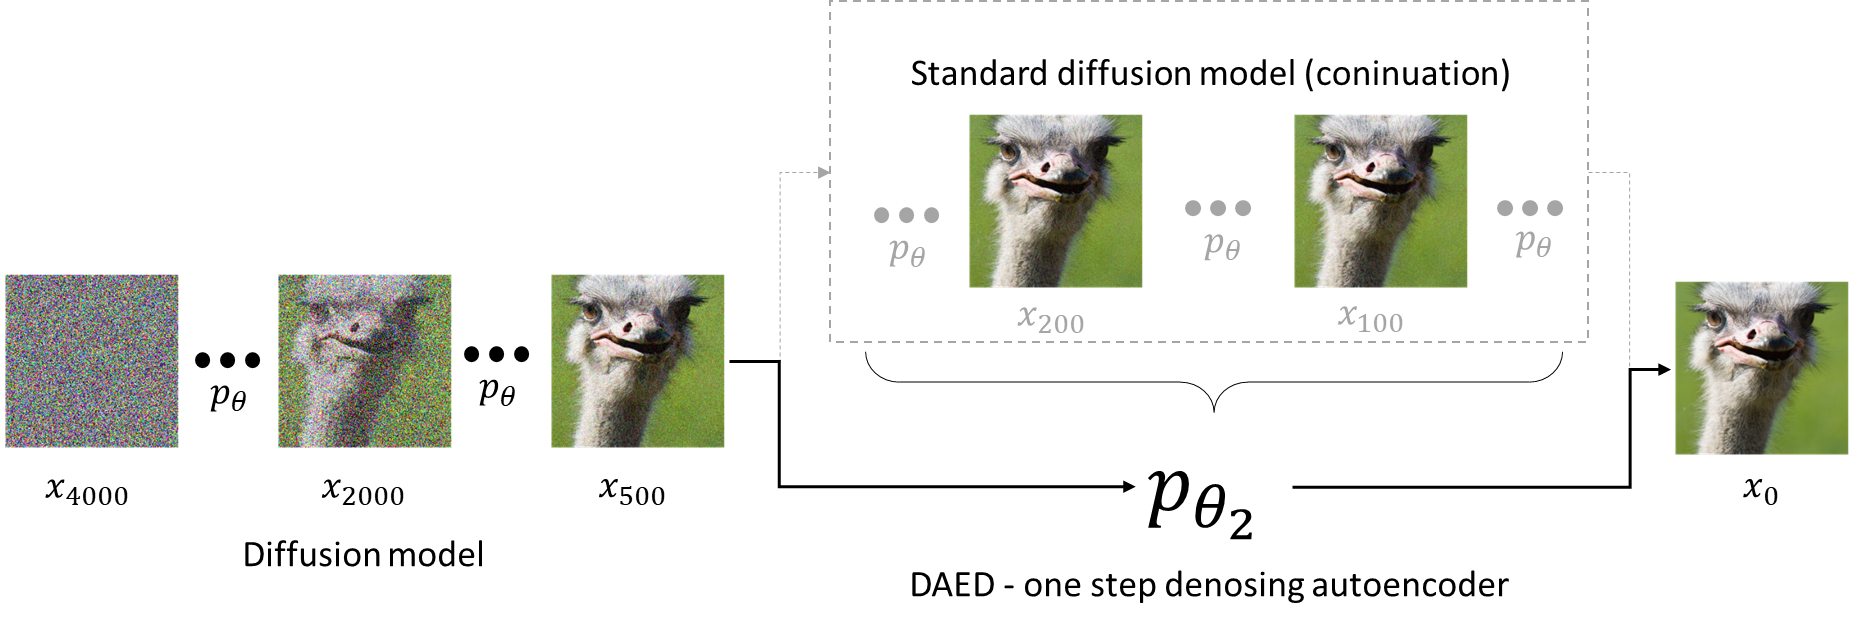
\includegraphics[width=.99\linewidth]{pics/4_daed/teaser.png}
	\caption{Overview of the proposed Denoising Auto-Encoder with Diffusion (DAED). To validate our hypothesis that DDGMs can be understood as a composition of a \emph{generator} and \emph{denoiser}, we propose to explicitly model the denoising part with a separate denoising autoencoder.}
	\label{fig:teaser}
% 	\vskip  -4pt
\end{figure}


In particular, we aim to answer the following three questions in this paper: 
\textbf{(i)} Is there a transition in the functionality of the backward diffusion process that switches from generating to denoising?
\textbf{(ii)} How does this split of functionality affect the performance? 
\textbf{(iii)} Does the denoising part in DDGMs generalize to other data distributions? 
As a result, the contribution of the paper is threefold:
\begin{itemize}
    \item First, we analyze the noise distribution in the forward diffusion process and how steps of the diffusion process are correlated with the reconstruction error.
    \item Second, based on our analysis, we postulate that DDGMs are composed of two parts: a \textit{denoiser} and a \textit{generator}. As a result, we propose a new class of models that consist of a Denoising Auto-Encoder and a Diffusion-based generator shortened as DAED. \ours{} could be considered as a variation of DDGMs with an explicit split into the denoising part and the generating part. 
    \item Third, we empirically assess the performance of DDGMs and \ours{} on three datasets (FashionMNIST, CIFAR10, CelebA) in terms of data generation and transferability (i.e., how DDGMs behave on different data distribution).
\end{itemize}
